
\documentclass[article]{memoir}

% ----- Packages -----
\usepackage{amsmath}
\usepackage{amsfonts}
\usepackage{amssymb}
% Must come after amsmath.
%\usepackage{amsthm}

\usepackage{mathtools}
\usepackage{subdepth}
\usepackage{dsfont}
\usepackage{flafter}
\usepackage{graphicx}
\usepackage{listings}

% ----- Page -----
\setlrmarginsandblock{1in}{1in}{*}
\setulmarginsandblock{1in}{1in}{*}
\checkandfixthelayout

\makepagestyle{name}
    \makeevenhead{name}{\textsl\thetitle}{}
    {\textsl{\thepage\ of \thelastpage\ --- Nick Ulle}}
    \makeoddhead{name}{\textsl\thetitle}{}
    {\textsl{\thepage\ of \thelastpage\ --- Nick Ulle}}
\makepagestyle{no-name}
    \makeevenhead{no-name}{\textsl\thetitle}{}
    {\textsl{\thepage\ of \thelastpage}}
    \makeoddhead{no-name}{\textsl\thetitle}{}
    {\textsl{\thepage\ of \thelastpage}}

% ----- Floats -----
\changecaptionwidth
\captionwidth{0.6\textwidth}
\setfloatadjustment{table}{\centering}
\setfloatadjustment{figure}{\centering}

\newsubfloat{table}
\newsubfloat{figure}

%\setFloatBlockFor{chapter}

% ----- Listings -----
\lstset{basicstyle = \ttfamily, numberstyle = \tiny, stepnumber = 2}

% ----- Commands -----
% Unbind some things that are never useful.
    % Built-in probability operator:
\let\Pr\relax%
    % Slashed O:
\let\O\relax%

% Set up sentence-ending ellipses.
\def\ldotsplus{\mathinner{\ldotp\ldotp\ldotp\ldotp}}
\def\fourdots{\relax\ifmmode\ldotsplus\else$\m@th \ldotsplus\,$\fi}

% Use the nice phi.
\let\temp\phi
\let\phi\varphi
\let\varphi\temp


\DeclareMathOperator{\Pr}{\mathds{P}}
\DeclareMathOperator{\E}{\mathds{E}}
\DeclareMathOperator{\Var}{Var}
\DeclareMathOperator{\Cov}{Cov}
\DeclareMathOperator{\Cor}{Cor}
\DeclareMathOperator{\eul}{e}
\DeclareMathOperator{\1}{\mathbf{1}}
\DeclareMathOperator{\sign}{sign}
\DeclareMathOperator{\diag}{diag}
\DeclareMathOperator{\tr}{tr}
\DeclareMathOperator*{\argmin}{argmin}
\DeclareMathOperator*{\argmax}{argmax}
\DeclareMathOperator{\O}{\mathcal{O}}
%\DeclareMathOperator{\N}{N}
%\DeclareMathOperator{\F}{F}
%\DeclareMathOperator{\Wishart}{W}

\newcommand{\abs}[1]{\lvert#1\rvert}
\newcommand{\norm}[1]{\lVert#1\rVert}
\newcommand{\ceil}[1]{\lceil#1\rceil}
\newcommand{\floor}[1]{\lfloor#1\rfloor}
\newcommand{\df}{\,\mathrm{d}}
\newcommand{\pd}[2][]{\frac{\partial#1}{\partial#2}}
\newcommand{\dv}[2][]{\frac{\mathrm{d}#1}{\mathrm{d}#2}}
\newcommand{\inD}{\mathop{\overset{\mathrm{d}}{\longrightarrow}}}
\newcommand{\inP}{\mathop{\overset{\Pr}{\longrightarrow}}}
\newcommand{\qed}{\hfill \ensuremath{\square}}
\newcommand{\T}{^\mathsf{T}}
\newcommand{\C}{^\mathsf{C}}
\newcommand{\io}{\text{ i.o.}}
\newcommand{\ev}{\text{ ev.}}
\newcommand{\dist}[1]{\operatorname{#1}}
\newcommand{\iid}{\overset{\mathrm{iid}}{\sim}}
\newcommand{\on}[1]{\operatorname{\mathds{1}}\!\left\{#1\right\}}
\newcommand{\ind}{\protect\mathpalette{\protect\independenT}{\perp}}

\def\independenT#1#2{\mathrel{\rlap{$#1#2$}\mkern4mu{#1#2}}}


\pagestyle{name}
\title{STA 250: Homework 1}

\begin{document}
\chapter{Report}
\begin{enumerate}
\item
    \begin{enumerate}
    \item
    Suppose $p(x_1, x_2)$ is a target density.
    Let $q(y \vert x)$ denote the density of transitioning from state $x$ to
    state $y$ in the Gibbs sampler. 
    For the two-component Gibbs sampler, $x$ and $y$ are two-dimensional.
    Then
    \begin{align*}
        q(y \vert x)
        &=
        q(y_1, y_2 \vert x_1, x_2)
        \\ &=
        q(y_2 \vert x_1, x_2, y_1) q(y_1 \vert x_1, x_2)
        \\ &=
        p(y_2 \vert x_1, x_2, y_1) p(y_1 \vert x_1, x_2)
        \\ &=
        p(y_1, y_2 \vert x_1, x_2).
    \end{align*}
    Integrating this against the target density,
    \begin{align*}
        \int p(x) p(y \vert x) \;dx
        &=
        \iint p(x_1, x_2) p(y_1, y_2 \vert x_1, x_2) \;dx_1 \;dx_2
        \\ &=
        \iint p(y_1, y_2, x_1, x_2) \;dx_1 \;dx_2
        \\ &=
        p(y_1, y_2).
    \end{align*}
    Therefore the target density is a stationary distribution of the Markov
    chain generated by the Gibbs sampler. Since the chain is ergodic, it is the
    unique stationary distribution.

    \item
    The $p$-dimensional case is similar to the two-dimensional case shown in
    part (a). In particular, for $p$-dimensional vectors $x$ and $y$,
    \begin{align*}
        q(y \vert x)
        &=
        p(y_k \vert x, y_{[1:k - 1]}) 
        p(y_{k-1} \vert x, y_{[1:k-2]})
        \ldots
        p(y_1 \vert x)
        \\ &=
        p(y \vert x).
    \end{align*}
    Then by integrating as before,
    \begin{align*}
        \int p(x) q(y \vert x) \;dx
        &=
        \int p(x) p(y \vert x) \;dx
        \\ &=
        \int p(y, x) \;dx
        \\ &=
        p(y).
    \end{align*}
    Thus the Markov chain converges to the target distribution.
    \end{enumerate}

\item
We are given the logistic regression model where
\[
    y_i \vert \beta \sim
    \dist{Bin} \bigl( m_i, \logit^{-1}(x_i\T \beta) \bigr)
    \qquad\text{for}\qquad
    i = 1, \ldots, n
\]
are conditionally indpendent and $\beta \sim \dist{N}_p(\mu_0, \Sigma_0)$.
\begin{enumerate}[i)]
    \item
    The joint likelihood of the $y_i \vert \beta$ is
    \[
        p(y \vert \beta)
        =
        \prod_{i=1}^n \binom{m_i}{y_i}
        \Biggl[ \frac{\eul^{x_i\T \beta}}{1 + \eul^{x_i\T \beta}} \Biggr]^{y_i}
        \Biggl[ \frac{1}{1 + \eul^{x_i\T \beta}} \Biggr]^{m_i - y_i}
    \]
    and the prior is
    \[
        p(\beta)
        =
        (2\pi) \abs{\Sigma_0}^{-\frac{1}{2}}
        \exp \Bigl(
        -\frac{1}{2}(\beta - \mu_0)\T \Sigma_0^{-1} (\beta - \mu_0)
        \Bigr)
    \]
    Therefore the posterior likelihood (up to proportionality) is:
    \begin{align*}
        p(\beta \vert y)
        &\propto
        \exp \Bigl(
        -\frac{1}{2}(\beta - \mu_0)\T \Sigma_0^{-1} (\beta - \mu_0)
        \Bigr)
        \prod_{i=1}^n
        \Biggl[ \frac{\eul^{x_i\T \beta}}{1 + \eul^{x_i\T \beta}} \Biggr]^{y_i}
        \Biggl[ \frac{1}{1 + \eul^{x_i\T \beta}} \Biggr]^{m_i - y_i}
        \\ &\propto
        \exp \Bigl(
        -\frac{1}{2}(\beta - \mu_0)\T \Sigma_0^{-1} (\beta - \mu_0)
        \Bigr)
        \prod_{i=1}^n
        \Bigl( \eul^{x_i\T \beta} \Bigr)^{y_i}
        \Bigl( 1 + \eul^{x_i\T \beta} \Bigr)^{-m_i}
        \\ &\propto
        \exp \Bigl(
        -\frac{1}{2}(\beta - \mu_0)\T \Sigma_0^{-1} (\beta - \mu_0)
        + \sum_{i=1}^n x_i\T \beta y_i
        \Bigr)
        \prod_{i=1}^n
        \Bigl( 1 + \eul^{x_i\T \beta} \Bigr)^{-m_i}
    \end{align*}
    The logarithm of this was used in the code.

    \item
    For this part of the homework, a two-component Metropolis-Hastings
    algorithm was used to generate a sample from the posterior distribution.
    A bivariate normal distribution was used as the proposal distribution.
    The mean was set to the previous draw, and the covariance matrix was
    initially set to $0.005 I_2$, where $I_2$ denotes the $2 \times 2$ identity
    matrix.

    During the burn-in, the proposal covariance matrix was periodically
    rescaled by
    \[
        \eul^{1.25 (\alpha - 0.4)}
    \]
    where $\alpha$ denotes the current acceptance rate. 
    This rescaling operation occured every $100$ iterations (until the end of
    the burn-in).

    The sampler was run for a total of $11000$ iterations, with the first
    $1000$ of these discarded as burn-in.

    The starting scale for the covariance matrix, described above, was chosen
    by trial-and-error. Various scales ($1, 0.5, 0.25, \ldots$) were tried
    until the chain had an acceptance rate of $35\%$ to $45\%$.

    \item
    The numerical coverage properties are shown in table~\ref{tab:coverage}.
    In general, the percentiles of the posterior sample seem to cover the
    true parameters about as often as theory predicts.

    \begin{table}[hbt]
    \begin{tabular}{ccc}
    \toprule
    Theoretical & $\beta_0$ & $\beta_1$ \\
    \midrule
    1\%  & 0.005 & 0.005 \\
    5\%  & 0.070 & 0.030 \\
    10\% & 0.105 & 0.070 \\
    25\% & 0.245 & 0.205 \\
    50\% & 0.515 & 0.470 \\
    75\% & 0.740 & 0.745 \\
    90\% & 0.885 & 0.875 \\
    95\% & 0.940 & 0.950 \\
    99\% & 0.990 & 1.000 \\
    \bottomrule
    \end{tabular}
    \caption{
        Numerical coverage of the posterior sample.
    }
    \label{tab:coverage}
    \end{table}

    \item
    The graph of the coverage properties is included as an attachment. Much
    like the table, it shows no serious deviations from what the theory
    predicts. The coverage lines fall almost entirely within the guiding bands.
    \end{enumerate}

\item
    \begin{enumerate}[i)]
    \item
    The breast cancer data was fit using Metropolis-Hastings-within-Gibbs,
    for $31000$ iterations, of which $1000$ were discarded as burn-in. A
    univariate normal distribution was used as the proposal distribution for
    each parameter. Different variances were used for each of the proposal
    distributions; these are documented in table~\ref{tab:var}. They were
    chosen by running the sampler with a very long burn-in until the acceptance
    rates stabilized (and the rescaling factors were close to 1).

        \begin{table}[bt]
        \begin{tabular}{cccccc}
        \toprule
        Area & Compactness & ConcavePts & Concavity & FracDim & Perimeter \\
        0.001 &  0.800 &  0.700 & 0.800 & 0.800 & 0.002 \\
        \midrule
        Radius & Smoothness & Symmetry & Texture & Intercept & \\ 
        0.020 & 0.800 & 0.700 & 0.020 & 0.500 & \\
        \bottomrule
        \end{tabular}
        \caption{
            Initial proposal variances.
        }
        \label{tab:var}
        \end{table}

    \FloatBlock
    \item
    The lag-1 autocorrelations of the posterior sample is shown in 
    table~\ref{tab:ac}.
    These seem distressingly high, and suggest that the sample may have a very
    small effective sample size.
        \begin{table}[hbt]
        \begin{tabular}{cccccc}
        \toprule
        Area & Compactness & ConcavePts & Concavity & FracDim & Perimeter \\
        0.7727 & 0.9063 & 0.9260 & 0.9736 & 0.8024 & 1.0000 \\
        \midrule
        Radius & Smoothness & Symmetry & Texture & Intercept & \\ 
        1.0000 & 0.8248 & 0.9162 & 0.9949 & 1.0000 & \\
        \bottomrule
        \end{tabular}
        \caption{
            Lag-1 autocorrelations of posterior sample.
        }
        \label{tab:ac}
        \end{table}

    \FloatBlock
    \item
    The posterior percentiles for the eleven elements of the parameter are
    shown in table~\ref{tab:pct}. The covariates most related to cancer
    diagnosis are likely to be those that do not have $0$ in their
    credible intervals. This is true for Concavity, Perimeter, Radius,
    and the intercept term.
        \begin{table}[hbt]
        \begin{tabular}{lrrrrr}
        \toprule
        & 5\% & 25\% & 50\% & 75\% & 95\% \\
        \midrule
        Area        & -0.0002 &  0.0000 & 0.0002  & 0.0003  & 0.0006 \\
        Compactness & -0.8253 &  0.1722 & 0.8731  & 1.5547  & 2.5726 \\
        ConcavePts  & -0.3097 &  0.6570 & 1.3826  & 2.0503  & 3.0590 \\
        Concavity   &  0.7649 &  1.7267 & 2.3728  & 3.0392  & 4.0082 \\
        FracDim     & -2.1082 & -1.1108 & -0.4145 & 0.2210  & 1.2238 \\
        Perimeter   &  0.1559 &  0.2488 & 0.2956  & 0.4457  & 0.5448 \\
        Radius      & -3.1480 & -2.4446 & -1.4905 & -1.1846 & -0.5935 \\
        Smoothness  & -1.8398 & -0.9053 & -0.2357 & 0.4638  & 1.3873 \\
        Symmetry    & -2.0280 & -1.1166 & -0.4512 & 0.1819  & 1.1068 \\
        Texture     & -0.0014 & 0.0239  & 0.0429  & 0.0619  & 0.0886 \\
        Intercept   & -8.6728 & -8.0006 & -7.5398 & -7.1144 & -6.5030 \\
        \bottomrule
        \end{tabular}
        \caption{
            Posterior percentiles for the eleven elements of the parameter.
        }
        \label{tab:pct}
        \end{table}

    \FloatBlock
    \item
    A posterior predictive check was performed for the mean response.
    $30000$ new data sets were simulated from the posterior sample.
    A histogram of the simulated mean responses is shown in 
    figure~\ref{fig:ppc}.
    The heavy red line indicates the true mean response.
    Based on the histogram, the model does fit the data reasonably well,
    because the true mean response falls near the center of the simulated mean
    responses.
        \begin{figure}[p]
        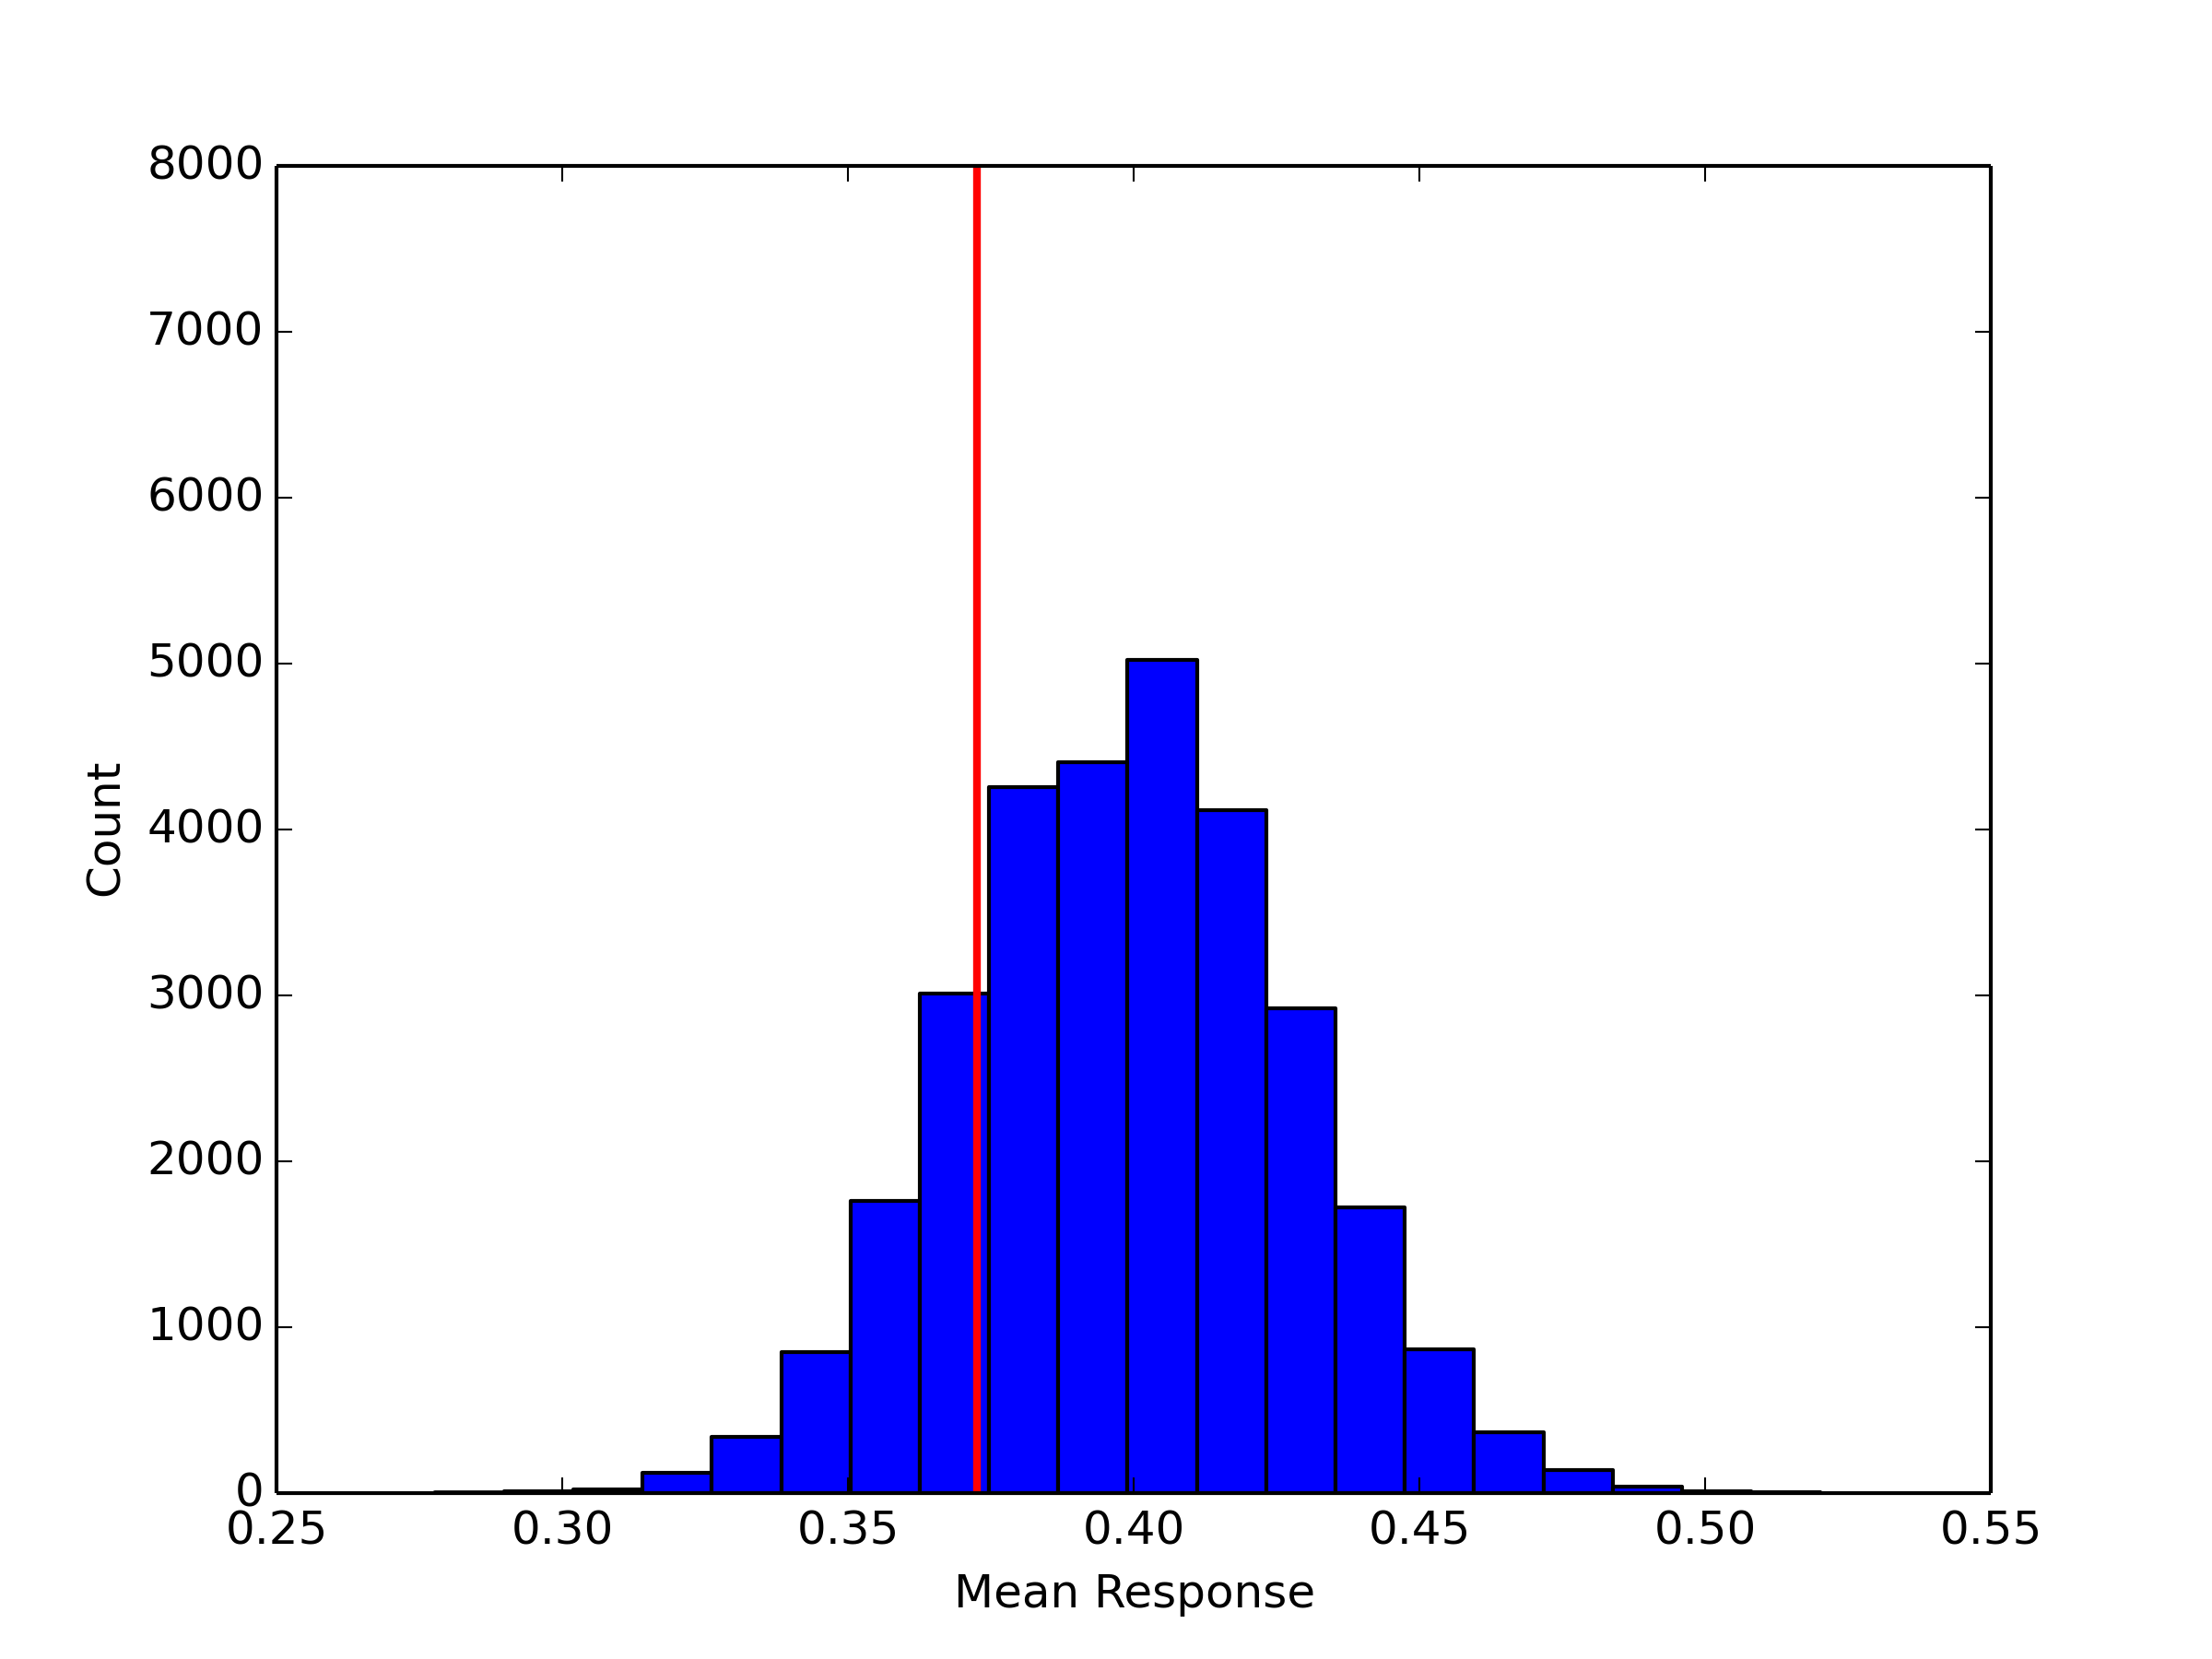
\includegraphics[width = 0.9\textwidth]{../BayesLogit/ppc_hist.png}
        \caption{
            Histogram of simulated mean response.
        }
        \label{fig:ppc}
        \end{figure}

    \item
    Based on the foregoing, doubt is cast on both the effectiveness of the
    posterior sample generated.
    In particular, the extremely high lag-1 autocorrelations suggest that an 
    even larger sample may be necessary to get a good representation of the 
    true posterior distribution. 
    Applying some kind of thinning may also help reduce autocorrelation.
    The posterior predictive check showed that the model itself is okay,
    but not excellent, for predicting the mean response. In this case it seems
    like domain-specific knowledge might allow for formulation of a better
    model, but the model fitted is a good naive model.
    \end{enumerate}
\end{enumerate}

\clearpage
\chapter{Source Code}
\lstinputlisting{../BayesLogit/BLR_fit.py}
\end{document}

